\hypertarget{group__poly}{
\section{Poly}
\label{group__poly}\index{Poly@{Poly}}
}


If your object is instatiated as a voice of a poly$\sim$ object, it is possible both to determine this context and to determine information about the specific voice.  


Collaboration diagram for Poly:\nopagebreak
\begin{figure}[H]
\begin{center}
\leavevmode
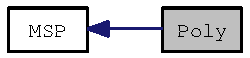
\includegraphics[width=78pt]{group__poly}
\end{center}
\end{figure}
If your object is instatiated as a voice of a poly$\sim$ object, it is possible both to determine this context and to determine information about the specific voice. This is done by querying the patcher in which your object exists for an associated object, and then calling methods on that object.


\begin{DoxyCode}
    t_object *patcher = NULL;
    t_max_err err = MAX_ERR_NONE;
    t_object *assoc = NULL;
    method m = NULL;
    long voices = -1;
    long index = -1;

    err = object_obex_lookup(x, gensym("#P"), &patcher);
    if (err == MAX_ERR_NONE) {
        object_method(patcher, gensym("getassoc"), &assoc);
        if (assoc) {
            post("found %s", object_classname(assoc)->s_name);

            voices = object_attr_getlong(assoc, gensym("voices"));
            post("total amount of voices: %ld", voices);

            if(m = zgetfn(assoc, gensym("getindex"))) 
                index = (long)(*m)(assoc, patcher);
            post("index: %ld", index);
        }   
    }       
\end{DoxyCode}
 